\documentclass[12pt,letterpaper,twoside]{article}

\newif\ifsolution\solutiontrue   % Include the solutions
%\newif\ifsolution\solutionfalse  % Exclude the solutions

\usepackage{cme213}
\usepackage{xcolor}
\usepackage{float}
\usepackage{graphicx}

\newcommand{\T}[1]{\text{\texttt{#1}}}
\newcommand{\V}[1]{\text{\textit{#1}}}

\begin{document}

{\centering \textbf{Final Report: Neural Networks on CUDA\\}}
\vspace*{-8pt}\noindent\rule{\linewidth}{1pt}

Goal of the final project is to implement a neural network with parallel 
matrix-matrix operations across four GPUs. Our neural network will be used
to identify digits from hand-written images from the MNIST dataset.

\paragraph{Part 1: Accelerated Matrix Multiplication} Idea: parallelize generalized
inplace matrix mulitplication $C = \alpha*A*B + \beta*C$ across cores of one GPU. We 
will be able to use this to excute multiple steps in the neural network's feed forward 
and back propagation operations.

\begin{figure}[!htbp]
    \centering
    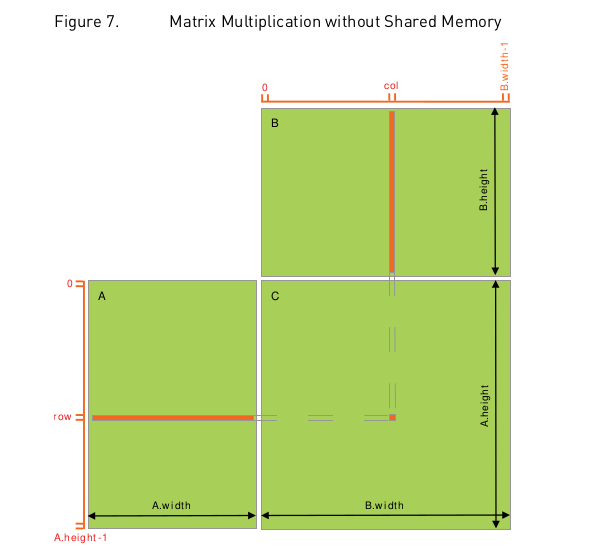
\includegraphics[scale=0.7]{gemm_naive.png}
    \caption{Naive matrix multiplication on GPU. Source: NVIDIA Programming Guide.}
\end{figure}

\begin{figure}[!htbp]
    \centering
    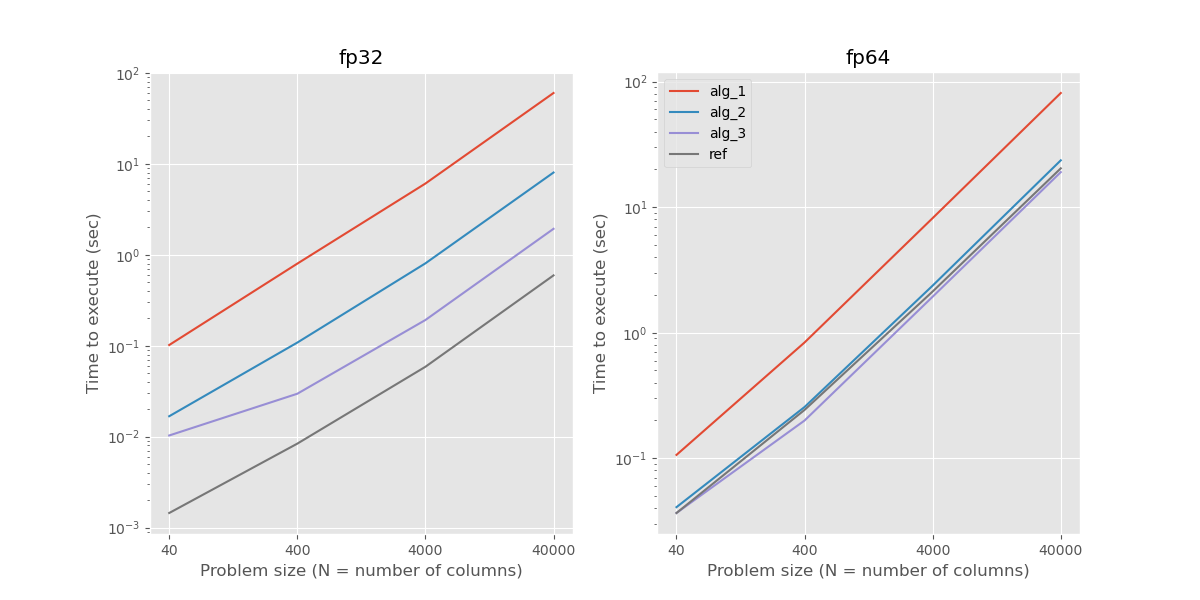
\includegraphics[scale=0.6]{speed_alg_vs_problem_size.png}
    \caption{Speed test of GEMM algorithms for float and double precision}
\end{figure}

Our first implementation is correct but naive and inefficient. We ask each thread to 
compute a single value of the output matrix C. This requires each thread to read an 
entire row from matrix A and column from matrix B, resulting in a lot of repeated 
global memory accesses for the same information as we work our way through the 
multiplication. See code sample below.

\begin{cpp}
/* 
Routine to perform an in-place GEMM, i.e., C := alpha*A*B + beta*C
*/
__global__ 
void kernelGEMM(nn_real* __restrict__ A, nn_real* __restrict__ B, 
        nn_real* __restrict__ C, nn_real alpha, nn_real beta, 
            int M, int N, int K) 
{
    // Each thread computes one element of C
    // by accumulating results into Cvalue
    nn_real Cvalue = 0;
    int row = blockIdx.y * blockDim.y + threadIdx.y;
    int col = blockIdx.x * blockDim.x + threadIdx.x;

    if (row < M && col < N) 
    {
        for (int e = 0; e < K; ++e) 
        Cvalue += A[row + M*e] * B[e +  K*col];	
        
    C[row + col*M] = alpha*Cvalue + beta*C[row + col*M];
    }
}
\end{cpp}

\begin{verbatim}
Output from code
----------------

*** Grading mode 4 ***

main -g 4
Number of MPI processes = 1
Number of CUDA devices = 4

Entering GEMM Benchmarking mode! Stand by.

Starting GEMM 1: M = 3200; N = 4000; K = 3136
GEMM matched with reference successfully! Rel diff = 1.00042e-07
Time for reference GEMM implementation: 0.0710125 seconds
Time for my GEMM implementation: 3.04307 seconds
Completed GEMM 1

Starting GEMM 2: M = 3200; N = 400; K = 4000
GEMM matched with reference successfully! Rel diff = 4.57243e-07
Time for reference GEMM implementation: 0.00806695 seconds
Time for my GEMM implementation: 0.389439 seconds
Completed GEMM 2

Starting GEMM 3: M = 3200; N = 40; K = 4000
GEMM matched with reference successfully! Rel diff = 7.29707e-07
Time for reference GEMM implementation: 0.00140079 seconds
Time for my GEMM implementation: 0.0438419 seconds
Completed GEMM 3

*** Tests are complete ***
\end{verbatim}

In subsequent implementations we will try to improve the performance of this 
generalized matrix multiplication algorithm. For example, one speed-up would be
to make use of shared memory. To do this, we could have each thread block compute
a sub-matrix (of size matching thread block dimensions) in the output matrix, with
just the required blocks from A and B read into shared memory. This allows us to 
make use of increased access speed of shared memory and take advantage of a more
coalesced global memory access pattern.


\paragraph{Part 2: Parallelize Neural Network (Single GPU)} Idea: training a neural
network involves repeatedly updating weights and biases at each layer through forward
and backwards propagation. Internally, these operations are mostly various adaptations
of genralized matrix multiplication! We want to take existing sequential code and 
parallelize each using cuda code from part 1.

\begin{itemize}
    \item \textbf{Feed forward.} Returns matrix \texttt{yc} from passing input images
    start to finish through the neural network layers. Here we parallelize the operations
    that compute activations of all neurons as well as the final softmax function. The 
    activations in aprticular are expensive to compute and essentially boil down to being 
    matrix-matrix multiplications. 

    \item \textbf{Back propagation.} Returns gradients \texttt{dW} and \texttt{db} from 
    passing the difference between \texttt{yc} and our target \texttt{y} back through the 
    neural network. Again we parallelize the core matrix operations involved, including
    transpose and matrix multiplication.

    \item \textbf{Gradient descent.} Returns updated neural network parameters (weights 
    \texttt{W} and biases \texttt{b}). This is a simple application of our graidents from 
    bakc propagation multiplied with a chosen learning rate. While I have parallelized this
    step, it is not clearly beneficial due to the MPI host-device back and forth required 
    to sum partial gradients across processes before gradient descent. 

\end{itemize}

\begin{verbatim}
Starting at Sat May 28 01:16:51 UTC 2022
Running on hosts: icmet04
Running on 1 nodes.
Running on 4 processors.
Current working directory is /home/jelc/cme213-para/project

Output from code
----------------

* Mode 1 *
mpirun -np 1 /home/jelc/cme213-para/project/main -g 1
Number of MPI processes = 1
Number of CUDA devices = 4
num_neuron=100, reg=0.0001, learning_rate=0.0005, num_epochs=40, batch_size=800
Loading training data
Training data information:
Size of x_train, N =  60000
Size of label_train = 60000

Start Parallel Training
Time for Parallel Training: 7.85949 seconds
Precision on validation set for parallel training = 0.829167

Grading mode on. Now checking for correctness...

Max norm of diff b/w seq and par: W[0]: 1.54722e-07, b[0]: 5.94913e-07
l2  norm of diff b/w seq and par: W[0]: 1.90251e-07, b[0]: 5.54432e-07
Max norm of diff b/w seq and par: W[1]: 1.5259e-07, b[1]: 1.91096e-07
l2  norm of diff b/w seq and par: W[1]: 1.55346e-07, b[1]: 2.35015e-07

* Mode 2 *
mpirun -np 1 /home/jelc/cme213-para/project/main -g 2
Number of MPI processes = 1
Number of CUDA devices = 4
num_neuron=100, reg=0.0001, learning_rate=0.001, num_epochs=10, batch_size=800
Loading training data
Training data information:
Size of x_train, N =  60000
Size of label_train = 60000

Start Parallel Training
Time for Parallel Training: 2.24912 seconds
Precision on validation set for parallel training = 0.756

Grading mode on. Now checking for correctness...

Max norm of diff b/w seq and par: W[0]: 8.94932e-08, b[0]: 4.61505e-07
l2  norm of diff b/w seq and par: W[0]: 1.23037e-07, b[0]: 4.71446e-07
Max norm of diff b/w seq and par: W[1]: 1.46356e-07, b[1]: 4.07745e-07
l2  norm of diff b/w seq and par: W[1]: 1.54429e-07, b[1]: 3.5195e-07

* Mode 3 *
mpirun -np 1 /home/jelc/cme213-para/project/main -g 3
Number of MPI processes = 1
Number of CUDA devices = 4
num_neuron=100, reg=0.0001, learning_rate=0.002, num_epochs=1, batch_size=800
Loading training data
Training data information:
Size of x_train, N =  60000
Size of label_train = 60000

Start Parallel Training
Time for Parallel Training: 0.56508 seconds
Precision on validation set for parallel training = 0.463667

Grading mode on. Now checking for correctness...

Max norm of diff b/w seq and par: W[0]: 3.62044e-08, b[0]: 4.51159e-07
l2  norm of diff b/w seq and par: W[0]: 5.70983e-08, b[0]: 3.23318e-07
Max norm of diff b/w seq and par: W[1]: 6.22334e-08, b[1]: 2.59939e-07
l2  norm of diff b/w seq and par: W[1]: 7.5405e-08, b[1]: 1.77756e-07

*** Summary ***

2400           1.40465e-07    1.45118e-07    6.03892e-07    1.9369e-07     1.75842e-07    1.51356e-07    5.24816e-07    2.36566e-07    
600            8.31383e-08    1.35914e-07    6.12333e-07    3.84295e-07    1.13652e-07    1.48703e-07    4.68868e-07    3.25847e-07    
60             3.33698e-08    6.31382e-08    4.08258e-07    2.66437e-07    5.36129e-08    7.22897e-08    3.02703e-07    1.9781e-07     

\end{verbatim}

\textbf{Remarks on debgugging.} This step required significant debugging effort given 
the inherent complexity of indexing many different variations of parallel matrix 
operations. My approach here was to add \texttt{\#if} and \texttt{\#endif} statements 
after each major step of the sequential algorithm and try to reproduce that step using 
my parallel code. To test whether the two implementations matched, I re-used existing 
\texttt{checkErrors} and \texttt{checkNNErrors} from the provided starter code test suite.


\paragraph{Part 3: Parallelize Training Batches (Multiple GPUs)} Idea: while each epoch 
needs to be executed sequentially, we can perform forwards and backwards propagation on 
batches within each epoch independently (and therefore in parallel). Our code from part 
2 should already make good use of hardware resources on a single GPU, however, in this 
project we have access to multiple GPUs! We use MPI to help coordinate sending different
training batches ('mini batches') to different GPUs as well as receiving back and 
aggregating outputs from each batch.

Steps implemented:
\begin{itemize}
    \item \textbf{MPI\_Scatter.} We use \texttt{MPI\_Scatter} to distribute mini batches
    of input images X and one-hot encoded target variables y across our 4 processes. 
    Each process then conducts its own feed forward and back propagation on its 
    respective minibatch of images and produces a set of partial gradients for 
    weights and biases.

    \item \textbf{MPI\_AllReduce.} We use \texttt{MPI\_AllReduce} to sum our partial 
    gradients that have been computed across our 4 processes together and broadcast 
    combined output back to all processes. To do this, we first needed to copy the 
    partial gradients from device to host of each process. Gradient descent can then 
    be computed on all processes (a bit wasteful) to update our neural network 
    parameters (weights and biases).

    Note: We needed to be careful to avoid accidentally scaling our gradients and 
    regularization term by the number of processes.
\end{itemize}

\begin{verbatim}

Output from code
----------------
* Mode 1 *
Time for Parallel Training: 6.56678 seconds

* Mode 2 *
Time for Parallel Training: 2.03137 seconds

* Mode 3 *
Time for Parallel Training: 0.69288 seconds
\end{verbatim}

The above runtime statistics show an improvement for mode 1 (epochs = 40) but actually
a decrease in performance for mode 3 (epochs = 1). This is because we incur a lot of
MPI setup overhead regardless but do not compute enough iterations to benefit from 
distributing across 4 GPUs (processes).


\paragraph{Part 4: Profiling Parallel Code} Idea: use NVIDIA's Nsight Systems and Nsight
Compute sofwtware tool to interrogate performance of code and assess how to improve.

\textbf{Nsight Systems:} Used this software to look across the whole program timeline 
and identify the largest relative sources of performance loss.

First takeaway from looking at Nsight Systems timeline was how expensive our 
\texttt{cudaMalloc} and \texttt{MPI\_Bcast} setup operations were compared to the 
neural network training itself. 

\begin{figure}[!htbp]
    \centering
    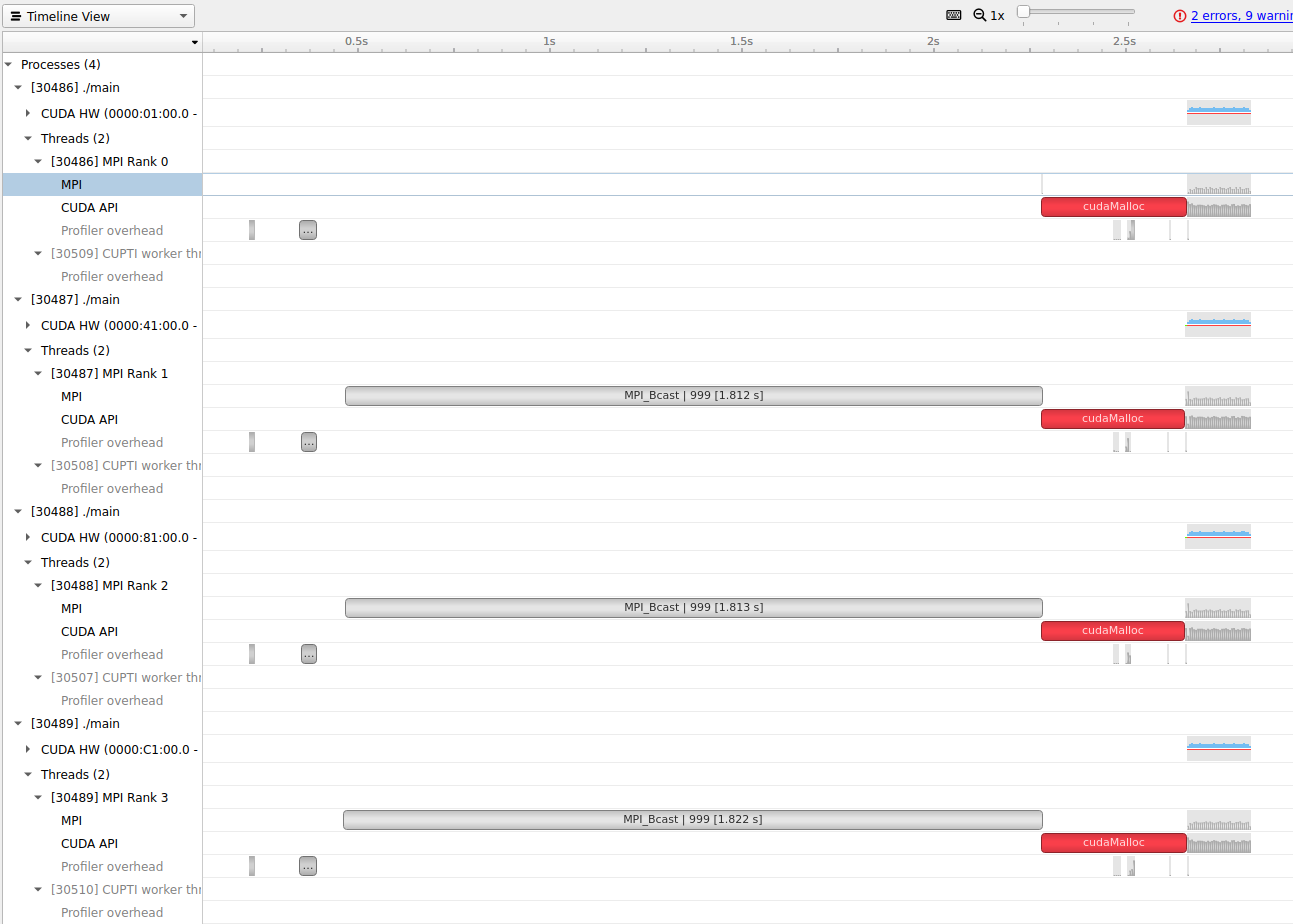
\includegraphics[scale=0.35]{nsight_systems_overview.png}
    \caption{Nsight Systems timeline of entire program for single epoch}
\end{figure}

Second takeaway was relative expense of \texttt{MPI\_Scatter} and \texttt{cudaMemcpy}
operations compared with our feed forward, back propagation and gradient descent kernels.
To me this highlights the importance to reducing the number of movements to and from the 
device, especially within the batch loops as is currently the case for X and y as well 
as gradients pre and post \texttt{MPI\_AllReduce}. It might even be worth eliminating 
the GPU parallel code for graident descent to avoid this!

\begin{figure}[!htbp]
    \centering
    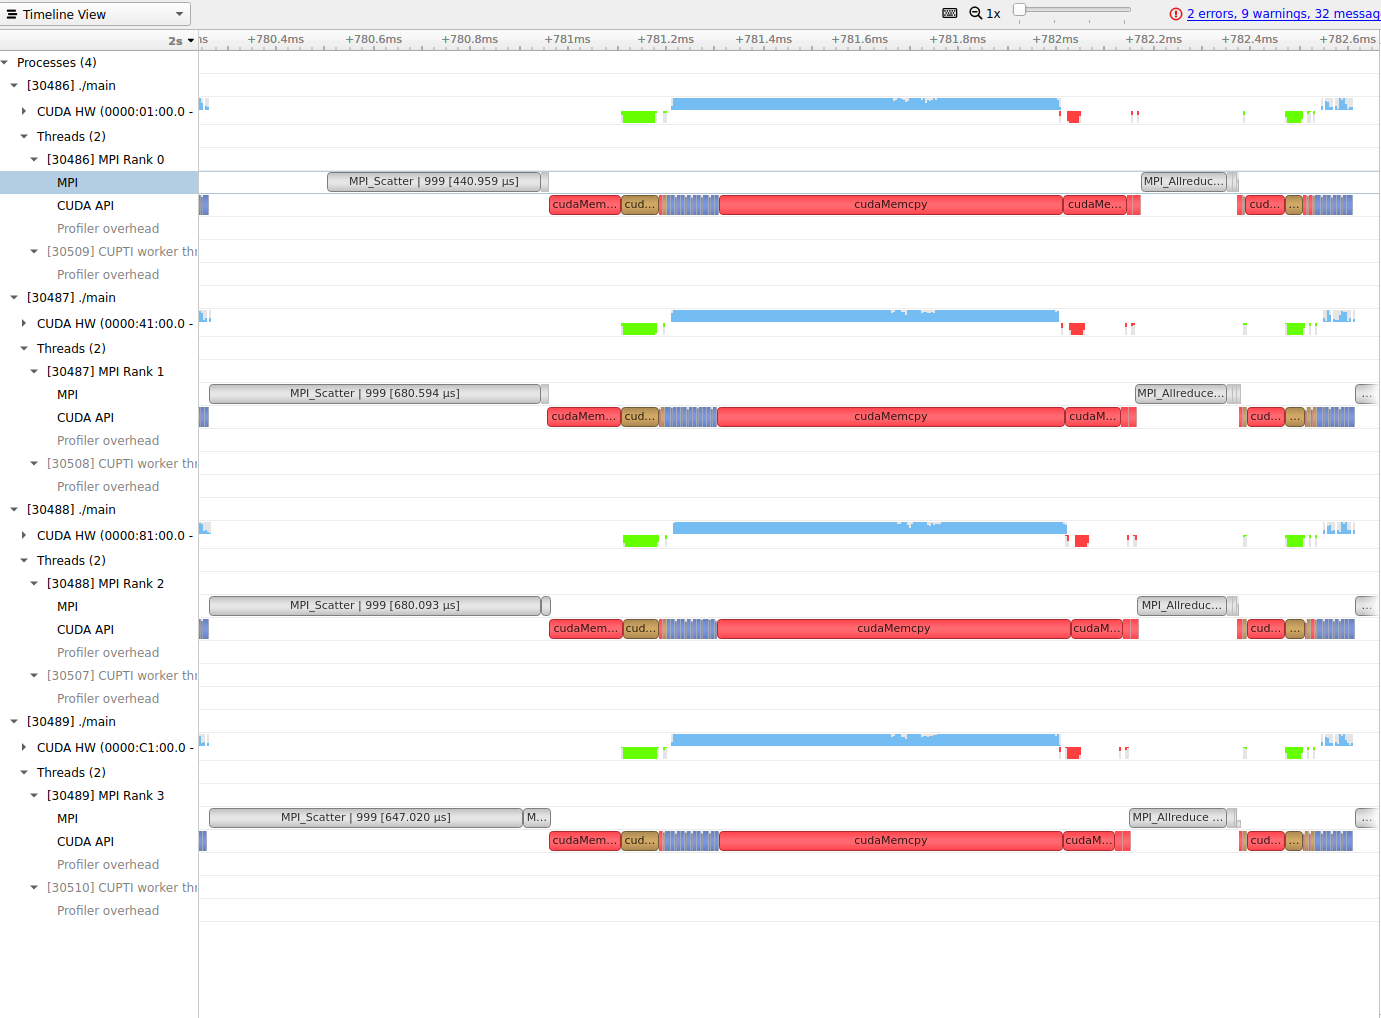
\includegraphics[scale=0.3]{nsight_systems_batch.png}
    \caption{Nsight Systems timeline for training of one image batch}
\end{figure}

Third takeaway was that our generalized matrix multiplication kernel was 3-4x the time 
cost of any other matrix operation kernel in our program. While this looks to be small 
here compared to data transfers, this becomes relevant when we want to train the neural 
network over 40 epochs.

\begin{figure}[!htbp]
    \centering
    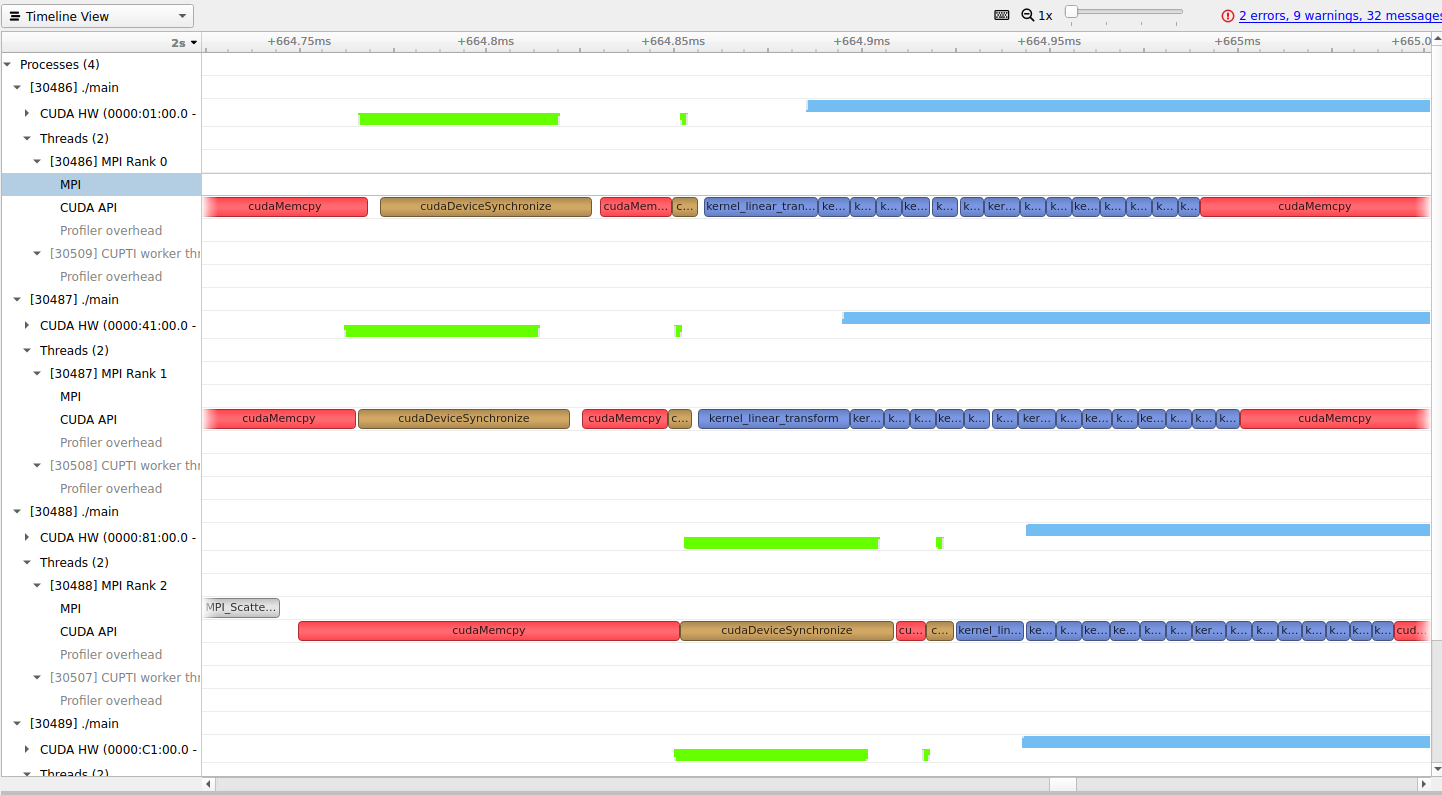
\includegraphics[scale=0.3]{nsight_systems_kernels.png}
    \caption{Nsight Systems relative time cost of all matrix kernels}
\end{figure}


\textbf{Nsight Compute:} Used this software to take a deeper look into the performance of 
individual kernels. In particular, our generalized matrix multiplication kernel.

Fourth takeaway was that we are still very much latency bound. Both our Compute and Memory
utilizations were far too low: 5.93\% and 22.56\% repectively. Goal here to is to increase 
utilization to ultimately increase arithmetic intensity. 

\begin{figure}[!htbp]
    \centering
    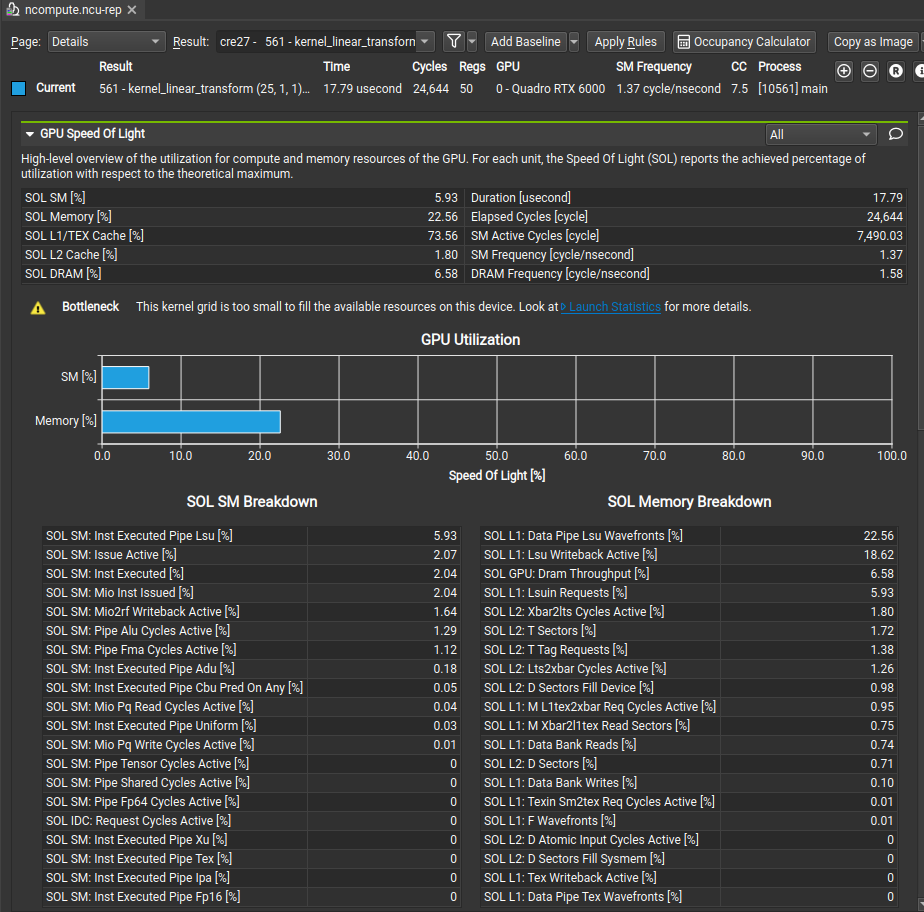
\includegraphics[scale=0.5]{nsight_compute_sol.png}
    \caption{Nsight Compute speed of light results for GEMM kernel}
\end{figure}

Fifth takeaway was we can immediately improve the launch configuration for this kernel.
We currently use a grid sizae of 25 which is far less than the GPU's 72 multiprocessors.
To improve we will want to increase the grid size to fully utilize available hardware.

\begin{figure}[!htbp]
    \centering
    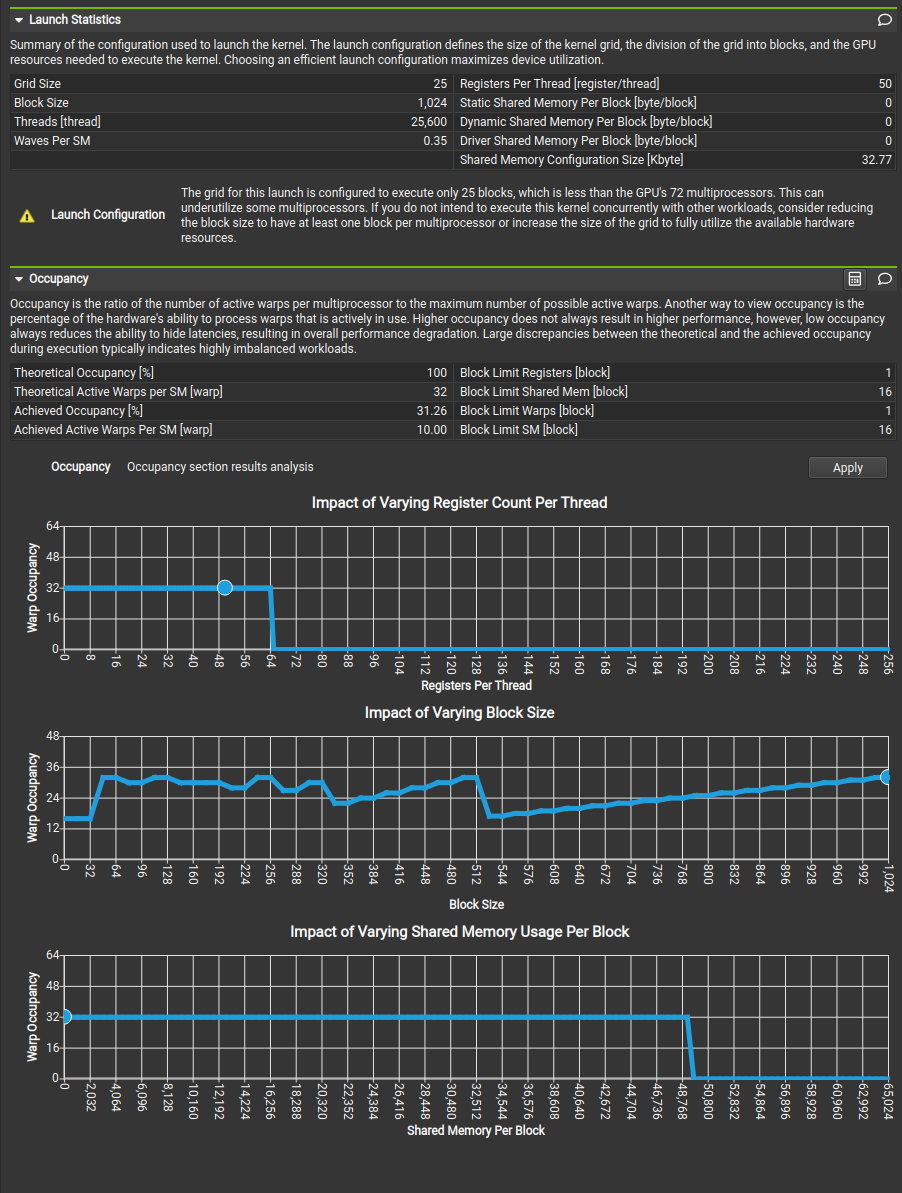
\includegraphics[scale=0.5]{nsight_compute_lao.png}
    \caption{Nsight Compute launch statistics and occupancy for GEMM kernel}
\end{figure}


Ideas to improve performance:
\begin{itemize}
    \item \textbf{Matrix multiplication.} Currently my generalized matrix multplication 
    is implemented such that each thread computes just one output value. This is super 
    inefficient since each thread needs to collect a bunch of data from global memory 
    (entire row of one matrix and column of the next) to do this one computation, 
    whereas if we asked the thread to compute a small block of values, it could 
    re-use much of its global memory request across these. 

    Additionally, we could store sections of the input matrices in shared memory to 
    make use of the increased bandwidth vs global memory associated with being 
    closer to the processing units.

    \item \textbf{Kernel usage.} I run a separate kernel for every individual compute 
    step. This means our kernels can be qutie generic (e.g. matrix multiplication, 
    matrix addition) which is great for debugging, but also means we spin up a lot 
    of separate kernels for each training cycle. It might be more effiicent to write 
    one kernel that handles multiple steps at once to reduce communication back and 
    forth (e.g. a feed forward kernel vs matrix multiplication kernel). 
    
    \item \textbf{Device memory allocation.} I allocate memory on the device for a 
    bunch of temporary variables to assist with intermediate calculations during 
    feed forward and back propagation steps. Looking at the profiler output, these 
    malloc steps are quite expensive and I imagine there are a number of optimization
    opportunities here to cut down on teh number of additional temporary variables
    by overwriting existing cache variables rather than write to new. 

    \item \textbf{Batching logic.} A more ambitious optimization might be to change 
    how I split work across my 4 GPUs (processes). Currently I divide each batch 
    into 'mini batches', however, instead I could think about dividing my model 
    parameters (weights and biases) across the different processes. 

\end{itemize}

\end{document}
